\documentclass[addpoints]{exam}

\usepackage{epic,array,ecltree,url}
\usepackage[nointegrals]{wasysym}


%These tell TeX which packages to use.
\usepackage{epsfig}
\usepackage{amsmath}
\usepackage{amsfonts}
\usepackage{amssymb}
\usepackage{amsxtra}
\usepackage{amsthm}
\usepackage{mlextra} % must be below ams packages
\usepackage{mathrsfs}
\usepackage[dvipsnames]{xcolor}
\usepackage{array}
\usepackage{graphicx}
\graphicspath{ {../art/} }
\usepackage{bm}
\usepackage{tikz}
\usepackage{multicol}

%Pagination stuff.
\setlength{\topmargin}{-.3 in}
\setlength{\oddsidemargin}{0in}
\setlength{\evensidemargin}{0in}
\setlength{\textheight}{9.in}
\setlength{\textwidth}{6.5in}

\newcommand{\twonode}{%
  \begingroup\normalfont
  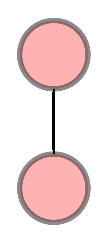
\includegraphics[height=\fontcharht\font`\b]{2nodetree.eps}%
  \endgroup
}

\newcommand{\tf}[1][{}]{%
\fillin[#1][0.25in]%
}
\noprintanswers
\unframedsolutions
\SolutionEmphasis{\itshape\small}
\SolutionEmphasis{\color{NavyBlue}}
\checkboxchar{$\Box$}
\checkedchar{$\blacksquare$}
\begin{document}


\noindent
\begin{tabular*}{\textwidth}{l @{\extracolsep{\fill}} r @{\extracolsep{6pt}} l}
{\large CS3920: Foundations of Computer Science} &  \makebox[3in]{\large Name:\enspace\hrulefill}\\
{\large May 14, 2018} & \\
{\large Quiz 3} & 
\end{tabular*}\\

\fbox{\fbox{\parbox{6in}{\textbf{Instructions}: Please answer the questions 
  below to the best of your ability. Be sure to show your work where appropriate. 
   This quiz is closed book, closed notes, closed computer. There are \numpoints\ 
   points in total. }}}\\
\begin{questions}
\question Let $A$ be the formula $p \lor \ngg p$.
\begin{parts}
\part[2] Which of the following correctly characterize(s) $A$? (Choose all that apply) 

\begin{oneparcheckboxes}
\CorrectChoice Valid
\CorrectChoice Satisfiable
\choice Falsifiable
\choice Unsatisfiable
\end{oneparcheckboxes}

\part[2] Which of the following correctly characterize(s) $\ngg A$? (Choose all that apply) 

\begin{oneparcheckboxes}
\choice Valid
\choice Satisfiable
\CorrectChoice Falsifiable
\CorrectChoice Unsatisfiable
\end{oneparcheckboxes}
\end{parts}

\question[2] Let $S$ be the formula $x \eqv y$. Write $S$ in clausal notation.
\begin{solution}
~\\
$x \imp y \land y \imp x$\\
$(\ngg x \lor y) \land (\ngg y \lor x)$\\
$\{\bar{x}y,x\bar{y}\}$
\end{solution}
\vspace{30mm}
\question Let $A$ be the formula $(p \imp \ngg (q \land \ngg p)) \lor (p \land q)$. 

\begin{parts}
\part[3] Write $A$ in conjunctive normal form.
\vspace{30mm}
\begin{solution}
~\\
$(\ngg p \lor \ngg (q \land \ngg p)) \lor (p \land q)$\\
$(\ngg p \lor \ngg q \lor p) \lor (p \land q)$\\
$(\ngg p \lor \ngg q \lor p \lor p) \land (\ngg p \lor \ngg q \lor p \lor q)$\\
$(\ngg p \lor \ngg q \lor p) \land (\ngg p \lor \ngg q \lor p \lor q)$\\

\end{solution}
\part[2] Show that $A$ is valid or give an interpretation that falsifies $A$.
\vspace{20mm}
\begin{solution}
$A$ is valid because \\
$(\ngg p \lor \ngg q \lor p) \land (\ngg p \lor \ngg q \lor p \lor q)$
$ = (\top \land \top) = \top$
\end{solution}

\end{parts}

\question Let $S, S'$ be propositional logic formulas in clausal form, 
 and $C, C' \in S$ clauses of $S$. 

\begin{parts}
\part[1] \tf[T] (T/F) If $S$ is satisfiable and $S' \subseteq S$, then $S'$ 
must be satisfiable.
\part[1] \tf[F] (T/F) If $C$ is satisfiable and $C' \subseteq C$, then $C'$
must be satisfiable.
\end{parts}

\vspace{10mm}
\question Let $S = \{r,pq\bar{r},st,uv\}$ and $S' = \{pq,st,uv\}$.

\begin{parts}
\part[1] \tf[T] (T/F) If $S$ is satisfiable then $r = T$.
\part[1] \tf[T] (T/F) If $S$ is satisfiable then $pq = \top$.
\end{parts}

\end{questions}
\end{document}


